Dany jest graf spójny nieskierowany $G = (V, E)$. 
Propagacja na takim grafie jest procesem stochastycznym. 
Zakładamy, że czas dla tego procesu jest dyskretny i mierzony w jednostkach naturalnych, zatem za zbiór chwil przyjmujemy $\mathbb{N}$.  
Niech $\mathcal{Q}$ będzie skończonym zbiorem stanów, jakie mogą przyjmować wierzchołki $G$.  
W każdej chwili $t \in \mathbb{N}$ każdy wierzchołek $v \in V$ znajduje się w pewnym stanie $Q \in \mathcal{Q}$.  
Nie będzie nas interesować przestrzeń zdarzeń elementarnych tego procesu.
Definiujemy realizacje zmiennej losową $\mathbf{X} : \mathbb{N}\times V \to \mathcal{Q}$ określającą stany wierzchołków grafu w czasie.
Mamy $\mathbf{X}_t(v) = Q$ wtedy i tylko wtedy, gdy wierzchołek $v$ w chwili $t$ znajduje się w stanie $Q$.  


\section{Model SI}

Model \textbf{Susceptible—Infected (SI)} opisuje propagację w sieci, w której każdy wierzchołek znajduje się w jednym z dwóch stanów: podatny ($S$) lub zainfekowany ($I$).  
Mamy więc $\mathcal{Q} = \{S, I\}$.  
Początkowo ustalone źródło $s \in V$ znajduje się w stanie $I$, natomiast pozostałe wierzchołki są w stanie $S$. 
A więc
\[
\mathbf{X}_0(v) =
\begin{cases}
I, & \text{jeśli } v = s,\\
S, & \text{jeśli } v \neq s.
\end{cases}
\]
W każdej jednostce czasu dowolny zainfekowany wierzchołek może zarazić każdego swojego sąsiada z prawdopodobieństwem $p$, dla ustalonego $p \in (0;1)$.  
Wierzchołek raz zainfekowany pozostaje w tym stanie na zawsze.  
W modelu SI liczba zainfekowanych wierzchołków jest funkcją niemalejącą w czasie.  
Dla uproszczenia notacji kładziemy 
\[
    q=1-p,\quad \mathcal{S}_t=\{v\in V: \mathbf{X}_t(v) = S\}, \quad \mathcal{I}_t=\{v\in V: \mathbf{X}_t(v) = I\}, \quad i_v=|\mathrm{N}(v) \cap \mathcal{I}_t|.
\]
Rozkład prawdopodobieństwa w tym modelu jest definiowany przez następujące zależności:
\begin{align*}
&\mathbb{P}[\mathbf{X}_{t+1}(v) = S \mid \mathbf{X}_t(v) = S] = q^{i_v}, \\[0.3em]
&\mathbb{P}[\mathbf{X}_{t+1}(v) = I \mid \mathbf{X}_t(v) = S] = 1 - q^{i_v}, \\[0.3em]
&\mathbb{P}[\mathbf{X}_{t+1}(v) = S \mid \mathbf{X}_t(v) = I] = 0, \\[0.3em]
&\mathbb{P}[\mathbf{X}_{t+1}(v) = I \mid \mathbf{X}_t(v) = I] = 1.
\end{align*}
Zdefiniujmy teraz zmienne losowe opisujące istotne dla nas własności.  
Dla każdego $v \in V$ definiujemy zmienną $X_v$ określającą chwilę czasu zarażenia wierzchołka $v$.  
Formalnie
\[
    X_v = \min \{ t \in \mathbb{N} : v \in \mathcal{I}_t \}.
\]
Jeśli taka chwila nie istnieje (tzn.\ w danym przebiegu procesu wierzchołek $v$ nigdy się nie zarazi), to przyjmujemy $X_v = \infty$.  
Później udowodnimy (\cref{theorem:total_infection}), że w modelu SI mamy $\mathbb{P}[X_v=\infty]=0$. 
Wyznaczenie rozkładu $X_v$ jak i $\mathbb{E}[X_v]$ da nam sporo informacji o propagacji na grafie w zależności od jego topologii.
Następnie dla każdego $t\in\mathbb{N}$ definiujemy zmienną losową $Y_t$ oznaczającą liczbę zainfekowanych wierzchołków w chwili $t$. 
Zatem
\[
    Y_t = |\mathcal{I}_t|.
\]
Interesować nas będzie rozkład prawdopodobieństwa $Y_t$ oraz wartość oczekiwana $\mathbb{E}[Y_t]$.
Pokażemy, że $\mathbb{E}[Y_t] \to |V|$ wraz z $t\to\infty$ (\cref{theorem:total_infection}). 
Dlatego też nie będziemy badać asymptotyki $\mathbb{E}[Y_t]$ względem $t$.
Dodatkowo definiujemy zmienną $Z$ opisującą czas całkowitego zarażenia grafu:
\[
    Z = \min \{ t \in \mathbb{N} : \mathcal{I}_t = V\}.
\]
Jeśli ta sytuacją nigdy nie nastąpi to $Z=\infty$.
Dla propagacji SI zainfekowanie całego grafu jest jednakże zdarzeniem pewnym. 
Wyznacznie rozkładu $Z$ oraz jej wartości oczekiwanej dla konkretnych rodzin grafów będzie głównym celem w tym modelu.


\begin{figure}[ht]
\centering 
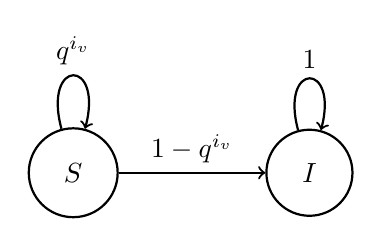
\begin{tikzpicture}[scale=1.5, node distance=3cm]
    \node[circle, draw, thick, inner sep=8pt, minimum size=20pt] (S) {$S$};
    \node[circle, draw, thick, inner sep=8pt, minimum size=20pt] (I) [right of=S] {$I$};
    \draw[->, thick, loop above] (S) to node[above] {$q^{i_v}$} (S);
    \draw[->, thick, loop above] (I) to node[above] {$1$} (I);
    \draw[->, thick] (S) to node[above] {$1-q^{i_v}$} (I);
\end{tikzpicture}
\caption{Diagram przejść dla modelu SI.}
\end{figure}


\section{Model SIR}

Model \textbf{Susceptible—Infected—Recovered (SIR)} rozszerza model SI o dodanie trzeciego stanu.  
Stanem tym jest $R$ (Recovered). 
W tym modelu mamy $\mathcal{Q} = \{S, I, R\}$.  
Stan $R$ jest pochłaniający — wierzchołek, który wyzdrowiał, nie może już ani się zarazić, ani nikogo zakazić.  
Zarażony wierzchołek może przejść z $I$ do stanu $R$ z prawdopodobieństwem $\alpha \in (0;1)$.  
Przyjmujemy, że w każda runda odbywa się w dwóch etapach.
W pierwszym z nich wierzchołki przekazują infekcje.
W drugim z nich te, które były już wcześnie zainfekowane mogą wyzdrowieć.
Dla uproszczenia notacji kładziemy 
\[
    \beta=1-\alpha,\quad \mathcal{R}_t=\{v\in V: \mathbf{X}_t(v) = R\}.
\]
Rozkład prawdopodobieństwa w tym modelu jest definiowany przez następujące zależności:
\begin{align*}
&\mathbb{P}[\mathbf{X}_{t+1}(v) = S \mid \mathbf{X}_t(v) = S] = q^{i_v}, \\[0.3em]
&\mathbb{P}[\mathbf{X}_{t+1}(v) = I \mid \mathbf{X}_t(v) = S] = 1 - q^{i_v}, \\[0.3em]
&\mathbb{P}[\mathbf{X}_{t+1}(v) = R \mid \mathbf{X}_t(v) = S] = 0, \\[0.3em]
&\mathbb{P}[\mathbf{X}_{t+1}(v) = S \mid \mathbf{X}_t(v) = I] = 0, \\[0.3em]
&\mathbb{P}[\mathbf{X}_{t+1}(v) = I \mid \mathbf{X}_t(v) = I] = \beta, \\[0.3em]
&\mathbb{P}[\mathbf{X}_{t+1}(v) = R \mid \mathbf{X}_t(v) = I] = \alpha, \\[0.3em]
&\mathbb{P}[\mathbf{X}_{t+1}(v) = S \mid \mathbf{X}_t(v) = R] = 0, \\[0.3em]
&\mathbb{P}[\mathbf{X}_{t+1}(v) = I \mid \mathbf{X}_t(v) = R] = 0, \\[0.3em]
&\mathbb{P}[\mathbf{X}_{t+1}(v) = R \mid \mathbf{X}_t(v) = R] = 1.
\end{align*}
Tak jak poprzednio rozważmy zmienne 
\[
    X_v=\min\{t\in\mathbb{N}:v\in\mathcal{I}_t\}.
\]
W kontraście dla modelu SI zachodzi $\mathbb{P}[X_v=\infty]>0$ (\cref{theorem:infection_dies_out_SIR}).
Z tego powodu wartość oczekiwana $\mathbb{E}[X_v]=\infty$ niezależnie od struktury grafu.
Dlatego też poza rozkładem $X_v$ możemy wyznaczyć $\mathbb{E}[X_v|X_v<\infty]$.
Istnienie stanu $R$ narzuca pomysł rozważania podobnej zmiennej na pierwszy czas wyzdrowienia wierzchołka $v$.
Ale transmisja ze stanu $I$ do $R$ na pojedynczym wierzchołku jest rozkładem $\mathrm{Geo}(\alpha)$, a więc zmienna ta była by po prostu sumą rozkładu geometrycznego oraz $X_v$.
Z tego powodu tego nie będziemy jej rozważać. 
Zamiast rozważać liczbę tylko zainfekowanych lub tylko wyzdrowiałych wierzchołków będziemy rozważać liczbe niepodatnych wierzchołków po $t$ krokach.
Kładziemy więc
\[
    Y_t=|\mathcal{I}_t\cup\mathcal{R}_t|.
\]
Mamy $\mathbb{P}[\mathcal{I}_t=\varnothing]\to1$ wraz z $t\to\infty$ (\cref{theorem:infection_dies_out_SIR}) a więc możemy zdefiniować zmienną $Z$ oznaczającą czas wygaśnięcia infekcji.
Dla uproszczenia będziemy rozważać moment w którym żaden nowy wierzchołek nie może być zarażony.
Zatem
\[
    Z = \min\{t\in\mathbb{N}: \forall v\in\mathcal{I}_t \quad \mathcal{S}_t\cap\mathrm{N}(v)=\varnothing\}.
\]
Dodatkowo definiujemy zmienną $W$ będącą liczba finalnie wyzdrowiałych wierzchołków.
\[
    W = |\{v\in V : X_v < \infty\}|.
\]
Rozkłady $Z,W$ jak i ich wartości oczekiwane będą naszym głównym obiektem zainteresowań w tym modelu.

\begin{figure}[ht]
\centering 
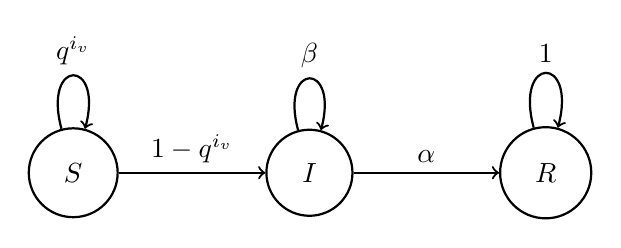
\begin{tikzpicture}[scale=1.5, node distance=3cm]
    \node[circle, draw, thick, inner sep=8pt, minimum size=20pt] (S) {$S$};
    \node[circle, draw, thick, inner sep=8pt, minimum size=20pt] (I) [right of=S] {$I$};
    \node[circle, draw, thick, inner sep=8pt, minimum size=20pt] (R) [right of=I] {$R$};
    \draw[->, thick, loop above] (S) to node[above] {$q^{i_v}$} (S);
    \draw[->, thick, loop above] (I) to node[above] {$\beta$} (I);
    \draw[->, thick, loop above] (R) to node[above] {$1$} (R);
    \draw[->, thick] (S) to node[above] {$1-q^{i_v}$} (I);
    \draw[->, thick] (I) to node[above] {$\alpha$} (R);
\end{tikzpicture}
\caption{Diagram przejść dla modelu SIR.}
\end{figure}


\section{Model SIS}

Model \textbf{Susceptible—Infected—Susceptible (SIS)} rozszerza model SI o powracanie wierzchołków zarażonych do stanu podatnego.  
Wierzchołek zainfekowany może powrócić do stanu podatnego z prawdopodobieństwem $\alpha \in (0;1)$.  
Tutaj tak jak w SI mamy $\mathcal{Q} = \{S, I\}$.  
W modelu SIS liczba zainfekowanych wierzchołków może oscylować w czasie i nie musi osiągnąć stanu pełnego zakażenia.  
Dla uproszczenia notacji kładziemy $\beta=1-\alpha$.  
Każda runda składa się z dwóch faz.
W pierwszej z nich wierzchołki zarażone próbują przekazać infekcje.
Natomiast w drugiej te zarażone wierzchołki, które były juz zarażone przez fazą pierwszą, mogą powrócić w stan podatności
Jest to odzwierciedlenie naturalnego stanu rzeczy.
Jeśli ktoś zostanie zakażony chorobą to nie może wyzdrowieć szybciej niż jego zakaziciel.  
Rozkład prawdopodobieństwa w tym modelu jest definiowany przez następujące zależności:
\begin{align*}
&\mathbb{P}[\mathbf{X}_{t+1}(v) = S \mid \mathbf{X}_t(v) = S] = q^{i_v}, \\[0.3em]
&\mathbb{P}[\mathbf{X}_{t+1}(v) = I \mid \mathbf{X}_t(v) = S] = 1 - q^{i_v}, \\[0.3em]
&\mathbb{P}[\mathbf{X}_{t+1}(v) = S \mid \mathbf{X}_t(v) = I] = \alpha, \\[0.3em]
&\mathbb{P}[\mathbf{X}_{t+1}(v) = I \mid \mathbf{X}_t(v) = I] = \beta.
\end{align*}
Zmienne losowe opisujące istotne własności są tutaj podobne jak w modelu SI.  
Dla każdego $v \in V$ kładziemy
\[
X_v = \min \{ t \in \mathbb{N} : v \in \mathcal{I}_t \},
\]
oraz dla $t\in\mathbb{N}$ definiujemy 
\[
    Y_t = |\mathcal{I}_t|.
\]
Wygaśnięcie infekcji zachodzi z prawdopodobieństwem $1$ (\cref{theorem:infection_dies_out_SIS}).
A więc definiujemy zmienną losową opisującą czas wygaśnięcia infekcji:
\[
    Z = \min \{ t \in \mathbb{N} : \mathcal{I}_t = \varnothing\}.
\]
Mamy $\mathbb{P}[X_v=\infty] > 0$ a zatem interesować nas będzie $\mathbb{E}[X_v|X_v<\infty]$.
Dalej wykażemy, że $\mathbb{E}[Y_t]$ dążą do $0$. (\cref{theorem:infection_dies_out_SIS})
Dlatego też także nie będą nas interesować.
Skupimy się tylko na rozkładzie $Y_t$.
Jeśli chodzi o zmienną $Z$ to przyjrzyjmy się zarówno jej rozkładowi jak i wartości oczekiwanej.

\begin{figure}[ht]
\centering 
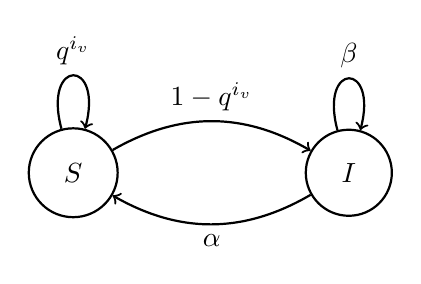
\begin{tikzpicture}[scale=1.5, node distance=3.5cm]
    \node[circle, draw, thick, inner sep=8pt, minimum size=20pt] (S) {$S$};
    \node[circle, draw, thick, inner sep=8pt, minimum size=20pt] (I) [right of=S] {$I$};
    \draw[->, thick, loop above] (S) to node[above] {$q^{i_v}$} (S);
    \draw[->, thick, loop above] (I) to node[above] {$\beta$} (I);
    \draw[->, thick, bend left=30] (S) to node[above] {$1-q^{i_v}$} (I);
    \draw[->, thick, bend left=30] (I) to node[below] {$\alpha$} (S);
\end{tikzpicture}
\caption{Diagram przejść dla modelu SIS.}
\end{figure}
